\documentclass[german,10pt]{book}      
\usepackage{makeidx}
\usepackage{babel}            % Sprachunterstuetzung
\usepackage{amsmath}          % AMS "Grundpaket"
\usepackage{amssymb,amsfonts,amsthm,amscd} 
\usepackage{mathrsfs}
\usepackage{rotating}
\usepackage{sidecap}
\usepackage{graphicx}
\usepackage{color}
\usepackage{fancybox}
\usepackage{tikz}
\usetikzlibrary{arrows,snakes,backgrounds}
\usepackage{hyperref}
\hypersetup{colorlinks=true,
                    linkcolor=blue,
                    filecolor=magenta,
                    urlcolor=cyan,
                    pdftitle={Overleaf Example},
                    pdfpagemode=FullScreen,}
%\newcommand{\hyperref}[1]{\ref{#1}}
%
\definecolor{Gray}{gray}{0.80}
\DeclareMathSymbol{,}{\mathord}{letters}{"3B}
%
\newcounter{num}
\renewcommand{\thenum}{\arabic{num}}
\newenvironment{anmerkungen}
   {\begin{list}{(\thenum)}{%
   \usecounter{num}%
   \leftmargin0pt
   \itemindent5pt
   \topsep0pt
   \labelwidth0pt}%
   }{\end{list}}
%
\renewcommand{\arraystretch}{1.15}                % in Formeln und Tabellen   
\renewcommand{\baselinestretch}{1.15}                 % 1.15 facher
                                                      % Zeilenabst.
\newcommand{\Anmerkung}[1]{{\begin{footnotesize}#1 \end{footnotesize}}\\[0.2cm]}
\newcommand{\comment}[1]{}
\setlength{\parindent}{0em}           % Nicht einruecken am Anfang der Zeile 

\setlength{\textwidth}{15.4cm}
\setlength{\textheight}{23.0cm}
\setlength{\oddsidemargin}{1.0mm} 
\setlength{\evensidemargin}{-6.5mm}
\setlength{\topmargin}{-10mm} 
\setlength{\headheight}{0mm}
\newcommand{\identity}{{\bf 1}}
%
\newcommand{\vs}{\vspace{0.3cm}}
\newcommand{\noi}{\noindent}
\newcommand{\leer}{}

\newcommand{\engl}[1]{[\textit{#1}]}
\parindent 1.2cm
\sloppy

         \begin{document}  \setcounter{chapter}{0}


\chapter{Physik des Klimas I\\Solarkonstante und Paleoklima}
\label{chap_Klima1}
% Kap x

\info{Thomas Filk}{30.03.2024}%
Unser Klima wird in erster Linie durch die Sonne bestimmt. Von ihr stammt die Energie,
die nahezu s\"amtliche dynamischen Vorg\"ange auf der Erde antreibt. 
Eine zweite Energiequelle besteht in Zerfallsprozessen radioaktiver Elemente im Erdinneren.
Diese Energieform k\"onnen wir jedoch f\"ur das Verst\"andnis des Klimas vernachl\"assigen.

Die Energieform, die in der Sonne durch Kernfusionsprozesse entsteht - streng genommen sollte
man nat\"urlich immer von \glqq Umwandlung\grqq\ sprechen, d.h., bei Kernfusionspozessen wird
Kernenergie in thermische (Bewegungs-)Energie, Strahlungsenergie sowie in Neutrinos umgewandelt -, 
erreicht uns in Form 
von elektromagnetischer Strahlung, haupts\"achlich im sichtbaren Bereich. Die Oberfl\"ache der
Sonne hat eine Temperatur von rund 5800\,Kelvin und die zugeh\"orige thermische Strahlung
hat ihr Maximum bei rund 500\,nm, das entspricht Licht im gr\"un-blauen Bereich. 

Der erste Abschnitt wird auf die Solarkonstante eingehen, d.h., die Menge an Energie, die pro
Zeiteinheit (Sekunde) und pro Fl\"acheneinheit (Quadratmeter) bei der Erde oberhalb der
Atmosph\"are ankommt. In diesem Zusammenhang gehen wir auch auf Ph\"anomene wie die Albedo
der Erde ein. Au\ss erdem betrachten wir verschiedene Faktoren, die in der Vergangenheit
einen Einfluss auf die Solarkonstante bzw.\ die Einstrahlung der Sonnenstrahlung auf die
Erde gehabt haben und damit unser Klima beeinflusst haben k\"onnten.
Schlie\ss lich betrachten wir auch kurz das Gebiet der Pal\"aoklimatologie, das sich mit
dem Klima im Verlauf der Erdgeschichte besch\"aftigt. 


\section{Die Solarkonstante}

Die Solarkonstante ist definiert als das langj\"ahrige Mittel der Intensit\"at pro Fl\"acheneinheit der 
Sonneneinstrahlung oberhalb der Erdatmosph\"are.\index{Solarkonstante} 
Die Intensit\"at ist dabei die Energie, die pro Sekunde 
auf eine bestimme Fl\"ache - in diesem Fall ein Quadratmeter senkrecht zur Strahlungsrichtung - trifft
(siehe Abb.\ \ref{fig_solar_constant}). 
Die IAU (International Astronomical Union) hat 2015 die Solarkonstante aufgrund neuerer
Messungen auf den Wert
\begin{equation}
               S = 1361\,{\rm J \cdot s^{-1} \cdot m^{-2}}
\end{equation}
festgelegt. In \"alteren B\"uchern findet man oft den Wert $S= 1367\,{\rm J \cdot s^{-1} \cdot m^{-2}}$, der
von 1982 bis 2015 G\"ultigkeit hatte. Heute misst man die Solarkonstante mit Satelliten, wobei die
gemessenen Intensit\"aten auf den mittleren Abstand Erde-Sonne - die Astronomische Einheit - 
umgerechnet wird.

\begin{SCfigure}[30][htb]
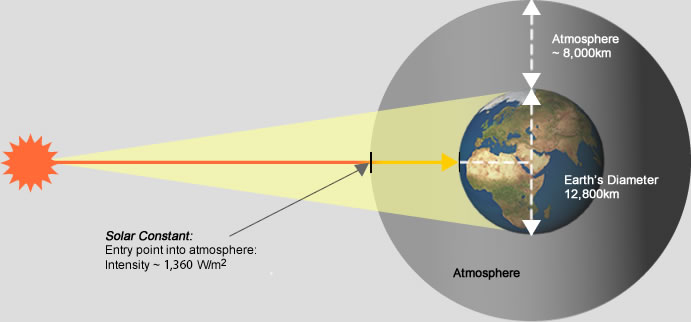
\includegraphics[scale=0.4]{./Bilder/solar-constant.jpg}
\caption{\label{fig_solar_constant}%
Definition der Solarkonstanten. Die gemessene Intensit\"at der Sonnenstrahlung
oberhalb der Erdatmosph\"are wird auf den mittleren Abstand Sonne-Erde umgerechnet.
(aus \cite{Solar})}
\end{SCfigure}


\subsection{Sonnenaktivit\"at}

Streng genommen handelt es sich bei der Solarkonstanten nicht um eine Naturkonstante. Sie unterliegt
kleinen Schwankungen.\index{11-Jahres-Zyklus der Sonne}\index{Sonnenzyklus} 
Eine winzige Schwankung entsteht durch den 11-Jahres-Zyklus der 
Sonnenaktivit\"at. Im sichtbaren Bereich machen diese Schwankungen aber nur rund 0,1\% aus. Lediglich
im UV- bzw.\ im R\"ontgen-Bereich k\"onnen diese Schwankungen wesentlich gr\"o\ss er sein, allerdings
wird diese Strahlung in h\"oheren Schichten unserer Atmosph\"are reflektiert bzw.\ absorbiert und 
erreicht den Erdboden gr\"o\ss tenteils nicht. Allerdings lassen sich Schwankungen in
der mittleren Jahrestemperatur von der Gr\"o\ss enordnung von $0,1^\circ$C mit einer Periode von 11
Jahren \"uber l\"angere Zeitr\"aume nachweisen. 
Au\ss erdem gab es in der Vergangenheit h\"aufiger Perioden, in denen die Sonne
insgesamt weniger aktiv war und die m\"oglicherweise zu kleinen Eiszeiten gef\"uhrt haben. Bekannt sind solche
Perioden in der Zeit zwischen dem 14.\ und 18.\ Jahrhundert (das sogenannte Sp\"orer-Minimum und das
Maunder-Minimum; wobei ein direkter Bezug zum Klima in dieser Periode immer noch umstritten ist), 
beispielsweise durch Wintergem\"alde von 
Pieter Bruegel dem \"Alteren und seinen S\"ohnen. 

Seit Beginn des 17.\ Jahrhunderts (seit der Erfindung des
Teleskops) wurden die Sonnenflecken direkt beobachtet, sodass es gute Aufzeichnungen
gibt. F\"ur die Perioden\index{Proxy!Sonnenaktivit\"at}\index{14-C@${}^{14}C}\index{10-Be@${}^{10}Be} 
davor eignen sich manche Isotopmessungen (z.B.\ ${}^{14}$C und ${}^{10}$Be).
Diese Isotope entstehen haupts\"achlich in der Atmosph\"are durch den Einfluss der kosmischen Strahlung, 
die wiederum durch eine starke Sonnenaktivit\"at und die damit verbundenen Sonnenwinde 
abgeschw\"acht wird. Dies f\"uhrt zu einer Korrelation zwischen der H\"aufigkeit dieser Isotope in
Bohrproben, die auf bestimmte Zeiten datiert werden k\"onnen, und der Sonnenaktivit\"at: H\"ohere
Isotopenanteile lassen auf geringere Sonnenaktivit\"at schlie\ss en, da zu diesen Zeiten die kosmische
Strahlung ungehinderter in die Atmosph\"are dringen konnte.

\subsection{Milankovi\'c-Zyklen}

F\"ur unser Klima\index{Milakonvi\`c, Milan}\index{Milankovi\`c-Zyklen}
relevante Schwankungen sind (vermutlich) die sogenannten Milankovi\'c-Zyklen, benannt nach
dem serbische Mathematiker Milutin Milankovi\'c (1879-1958). Hierbei handelt es sich um regelm\"a\ss ige
Oszillationen in den Parametern der Erdumlaufbahn um die Sonne. Diese Parameter sind
insbesondere die Exzentrizit\"at der Erdbahn, die Neigung der Erdachse und die
Pr\"azession der Erdachse.

\subsubsection{Die Exzentrizit\"at der Erdumlaufbahn} 

In einem reinen Zwei-K\"orper-Problem mit einer $1/r^2$-Kraft\index{Exzentrizit\"at}\index{Kepler-Problem, 2-K\"orper-}
(manchmal als nicht-relativistisches Kepler-Problem bezeichnet) bewegt sich ein leichter K\"orper (Erde)
um einen schweren K\"orper (Sonne) auf einer elliptischen Bahn, wobei sich der schwere K\"orper
in einem der Brennpunkte der Ellipse befindet. Dies gilt ganz allgemein f\"ur die Relativkoordinate
zwischen den beiden Himmelsk\"orpern, auch wenn die Masse des leichteren Himmelsk\"orpers
im Vergleich zu dem schwereren Himmelsk\"orper nicht vernachl\"assigt werden kann. In diesem Fall
bewegen sich die beiden K\"orper um einen gemeinsamen Schwerpunkt, der sich in einem der
Brennpunkte der Ellipse befindet.  

Durch den Einfluss der anderen Planeten, insbesondere Jupiter und Saturn, ver\"andert sich die 
Bahnkurve der Erde jedoch im Verlauf der Zeit. Insbesondere kann auch die Exzentrizit\"at der
elliptischen Bahn zwischen einer fast kreisf\"ormigen Erdumlaufbahn ($\epsilon = 0,0006$) und einer
schwach elliptischen Bahn ($\epsilon =0,058 $) variieren \cite{Wikipedia_Milankovic}. 
Diese Werte schwanken periodisch mit einer Periode von rund
405\,000 Jahren, wobei auch Unterzyklen von der Gr\"o\ss enordnung von 100\,000 Jahren existieren. 

Derzeit betr\"agt der Wert rund $\epsilon= 0,0167$, was einer Schwankung in der Entfernung zwischen
Erde und Sonne im Bereich zwischen\index{Exzentrizi\"atsschwankungen}
147,09 Millionen Kilometern und 152,10 Millionen Kilometern entspricht. Obwohl die Differenz in diesen
Werten nur rund 3.4\% ausmacht, bedeutet dies f\"ur die Intensit\"at der Sonnenstrahlung
eine Schwankung von rund 6,8\% im Verlauf eines Jahres \hyperref[Anm-1]{(1)}. 
Bei einer entsprechend gr\"o\ss eren Exzentrizit\"at sind auch diese 
Schwankungen gr\"o\ss er und k\"onnen bis zu 24\% ausmachen.

\subsubsection{Neigung der Erdachse} 

Im Vergleich zur Ekliptik, also der Ebene der Erdumlaufbahn\index{Erdachse!Neigung}
um die Sonne, ist die Drehachse der Erde um rund $23,5^\circ$ geneigt. Dieser Neigungswinkel
\"andert sich aufgrund der Einfl\"usse anderer Planeten mit einer Periode von rund 41.000 Jahren
und schwankt zwischen $22,1^\circ$ und $24,5^\circ$.

Auch diese Schwankung hat zun\"achst einen jahreszeitlichen Einfluss auf unser Klima: Ist der
Neigungswinkel gr\"o\ss er, ist der Unterschied im Einfallswinkel der Sonne zwischen Sommer und
Winter entsprechend gr\"o\ss er, d.h., die jahreszeitlichen Schwankungen fallen st\"arker aus. 
Das wiederum kann einen Einfluss darauf haben, wie stark Schnee- und Eisfl\"achen im Sommer
abtauen und sich somit zur\"uckbilden. Au\ss erdem haben diese Schwankungen einen Einfluss
auf verdunstende Wassermengen in h\"oheren Breitengraden und somit auf den dortigen Niederschlag, 
was sich beispielsweise im Winter auf erh\"ohten Schneezuwachs bei Gletschern auswirken kann. 

\subsubsection{Pr\"azession der Erdachse} 

Da die Erde keine ideale Kugelform hat sondern entlang der Erdachse\index{Praezession@Pr\"azession}
etwas abgeplattet ist, also entlang des \"Aquators etwas \glqq dicker\grqq\ als entlang von L\"angengraden
(der Abstand vom Erdzentrum zum Nord- bzw.\ S\"udpol ist um rund 21 Kilometer kleiner als der 
Abstand vom Erdzentrum zum \"Aquator, wobei hier f\"ur die Erde vereinfachend die\index{Erdform, Rotationsellipsoid} 
Form eines
Rotationsellipsoids angenommen wird). Der gravitative Einfluss von Sonne und Mond (in geringerem Ma\ss\
auch der von anderen Planeten, insbesondere Jupiter und Saturn) bewirkt ein Drehmoment, das 
die Erdachse aufrichten w\"urde, falls sich die Erde nicht drehte. Wegen der Drehimpulserhaltung wird
die Drehachse zur Seite gedreht und rotiert langsam um eine Senkrechte zur Erdbahn ((Bild!)).
Diese Drehung bezeichnet man als Pr\"azession. Sie hat eine Periode von rund 25\,800 Jahren.

Der Haupteffekt der Neigung der Erdachse sind die Jahreszeiten, die auf der Nord- und S\"udhalbkugel
der Erde um ein halbes Jahr relativ zueinander verschoben sind. Die Pr\"azession bewirkt, zusammen mit
den anderen Orbitalparametern, dass die Unterschiede zwischen den Jahreszeiten (insbesondere
zwischen Sommer und Winter) hinsichtlich ihrer Intensit\"at verschieden stark ausfallen k\"onnen.
Wenn beispielsweise die Elliptizit\"at der Erbahn (d.h.\ die Exzentrizit\"at) sehr gro\ss\ ist, kann
die Richtung der Erdachse relativ zu den Hauptachsen die Strahlungsunterschiede zwischen Sommer
und Winter entweder verst\"arken (wenn der Sommer mit dem Perihel zusammenf\"allt) oder
abschw\"achen (wenn Sommer mit dem Aphel zusammenf\"allt). 

Ein weiterer wesentlicher Faktor f\"ur das Klima ist, dass die Nordhalbkugel der Erde gr\"o\ss ere
Landmassen hat als die S\"udhalbkugel, die eine gr\"o\ss ere Wasserfl\"ache hat. Insofern spielt es
eine Rolle, ob die oben erw\"ahnte Verst\"arkung der Unterschiede zwischen Sommer und Winter
f\"ur die Nord- oder f\"ur die S\"udhalbkugel zutrifft.  

W\"ahrend man in der physikalischen und astrophysikalischen Literatur f\"ur die Pr\"azession der
Erde einen Wert von 25\,800 (oder aufgerundet 26\,000) Jahren findet, findet man in der
Literatur zur Klimaphysik bzw.\ zu den Milankovi\'c-Zyklen
oftmals einen Wert von 23\,000 Jahren. F\"ur die Physik (z.B.\ die
Bestimmung des Fr\"uhlingspunkts und den damit zusammenh\"angenden Jahreszeiten) ist
die Richtung der Erdachse relativ zur Sonne wichtig. F\"ur die Klimaforschung ist man eher an der
Richtung der Erdachse relativ zum Perihel bzw.\ Aphel interessiert. 
Wegen der Periheldrehung\index{Periheldrehung}
der Erde, verschieben sich diese Punkte aber langsam. Der kombinierte Effekt von 
Pr\"azession und Periheldrehung f\"uhrt zu der verk\"urzten Periode von 23\,000 Jahren. 


\subsection{Das Sonnenalter}

Auf sehr langen Zeitskalen nimmt die Solarkonstante zu: in 100 Millionen Jahren um rund 1\% 
\cite{Wikipedia_Solarkonstante}. Zu Beginn der Erdgeschichte betrug die 
Sonnenintensit\"at nur\index{Sonnenintensit\"at!in fr\"uheren Zeiten}\index{Fain young Sun paradox}
rund 70\% ihres heutigen Werts. Das Klima auf der Erde h\"atte somit wesentlich k\"alter sein m\"ussen
und alles Wasser auf der Erde h\"atte gefroren sein m\"ussen. Es gibt aber deutliche Hinweise
darauf, dass es insgesamt meist w\"armer auf der Erde gewesen ist. Dies bezeichnet man als
das  \textit{Faint young Sun paradox} \cite{Wikipedia_Faint}. Eine m\"ogliche L\"osung ist, dass der
Kohlendioxidgehalt der Atmosph\"are in fr\"uheren Zeiten (z.B.\ aufgrund von Vulkanismus)
wesentlich h\"oher war als heute. Diese Frage ist aber noch nicht endg\"ultig gekl\"art.

\section{Die Albedo}

Die Albedo\index{Albedo} 
ist ein Ma\ss\ daf\"ur, wie stark ein Gegenstand eine Strahlung reflektiert. Es ist so etwas
wie der totale elastische Wirkungsquerschnitt eines Gegenstands f\"ur elektromagnetische Strahlung. 
Allerdings handelt es sich nicht um eine Fl\"ache, sondern um ein Verh\"altnis: das Verh\"altnis
von reflektierter Intensit\"at zu eingestrahlter Intensit\"at. Man kann die Albedo als Funktion
der Wellenl\"ange bzw.\ der Frequenz betrachten (da es um die reflektierte Strahlung geht, soll die
Wellenl\"ange bzw.\ Frequenz erhalten bleiben), meist interessiert man sich aber f\"ur die
Summe \"uber das gesamte Spektrum. 

Wenn man ein Foto von der Erde betrachtet, aufgenommen von einem Satelliten oder, besser noch, 
von einer Raumsonde oder Rakete auf dem Weg zum Mond oder einem anderen Ort im Sonnensystem,   
ist alles, was man von der Erde sieht, reflektierte Strahlung (siehe Abb.\ \ref{fig_NASA_Welt}). 
Auf einem solchen Bild sieht man
sofort, welche Teile der Erde eine hohe und welche eine niedrige Albedo haben: Schnee- und Wolkenfelder
haben eine hohe Albedo, ebenso Eisfelder; Wasser und W\"alder haben eine sehr niedrige Albedo. 
Sand bzw.\ W\"uste oder Steppen haben eine mittlere Albedo. 

\begin{SCfigure}[30][htb]
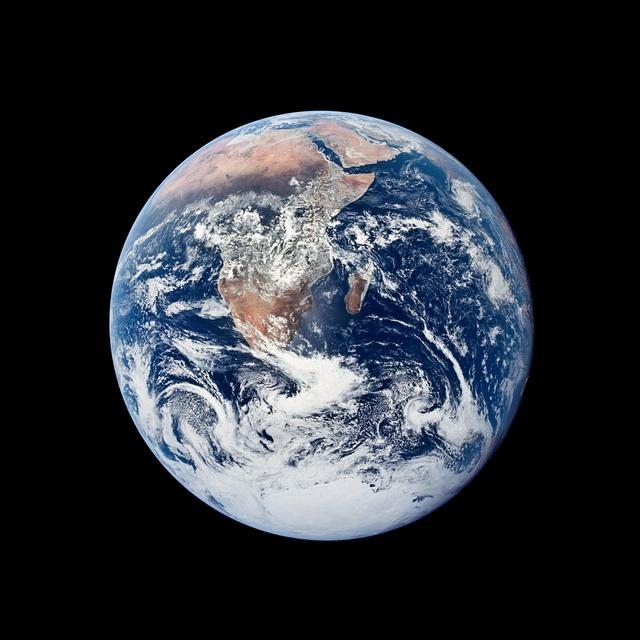
\includegraphics[trim=70 70 70 70, clip, width = 0.33\textwidth]{./Bilder/as17-Albedo-orig.jpg}
\caption{\label{fig_NASA_Welt}%
Die Erde, aufgenommen von der Crew der Apollo-17 Mission im Jahre 1972. Deutlich erkennbar sind
die Antarktis, der afrikanische Kontinent, die Insel Madagaskar und die saudi-arabische Halbinsel. Die sehr
stark reflektierenden Gebiete sind wei\ss, das sind Schnee- und Wolkenfl\"achen. Die W\"usten sind
deutlich heller als Waldgebiete oder Grasfl\"achen. 
Sehr dunkel sind die Meere. Diese Helligkeiten entsprechen der
Albedo der jeweiligen Fl\"achen. (aus \cite{NASA_World})}
\end{SCfigure}

Die Albedo hat einen sehr gro\ss en Einfluss auf unser Klima. Je gr\"o\ss er die Albedo eines
Planeten ist, umso geringer ist (bei gleichbleibenden anderen Faktoren) die Oberfl\"achenerw\"armung. 
W\"ahrend die Erde insgesamt eine Albedo von 0,3 hat, hat beispielsweise der Planet Venus\index{Albedo!Venus} 
aufgrund seiner dichten Wolkenschicht eine Albedo von 0,7. Obwohl Venus deutlich n\"aher an der Sonne
ist als die Erde und aus diesem Grunde eine doppelt so hohe Solarkonstante hat, w\"are ihre
Temperatur aufgrund der Albedo k\"uhler als die der Erde. Tats\"achlich ist ihre Oberfl\"achentemperatur 
jedoch wesentlich h\"oher (bei $460^\circ$C). Der Grund ist der Treibhauseffekt: Die Atmosph\"are
von Venus besteht zu 96\% aus Kohlendioxid.\index{Venus!Albedo}\index{Venus!Atmosph\"are}\index{Atmosph\"are!Venus} 

\section{Aufbau der Atmosph\"are}

Die Atmosph\"are der Erde\index{Erdatmosph\"are}\index{Atmosph\"are!Erde} 
wird in verschiedene Schichten unterteilt, von denen die untersten
drei Schichten - die Troposph\"are, die Stratosph\"are und die Mesosph\"are - den gr\"o\ss ten
Einfluss auf unser Klima haben. Sie sind durch ihre Temperaturgradienten definiert. Die beiden
dar\"uber liegenden Schichten - die Thermosph\"are (100--600\,km) und die Exosph\"are
(600--200\,000\,km) - haben keinen direkten Einfluss auf unser Wetter bzw.\ Klima. 

\subsection{Die Troposph\"are}

Die Troposph\"are\index{Troposph\"are} 
ist die unterste Atmosph\"arenschicht, in der sich nahezu alle Wettervorg\"ange
abspielen. Definiert ist sie durch einen negativen Temperaturgradienten, d.h., in dieser Schicht
nimmt die Temperatur mit der H\"ohe ab. Sie erstreckt sich an den Polen bis in eine H\"ohe von
rund 6--8\,km, in den Tropen bis zu einer H\"ohe von 12--18\,km. Im Durchschnitt hat sie eine
H\"ohe von 13\,km. 

Die Abnahme der Temperatur h\"angt mit der Druckabnahme zusammen. Der Druck nimmt
nahezu exponentiell mit der H\"ohe ab (dies gilt auch weit \"uber die Troposph\"are hinaus). Aus diesem
Grund dehnt sich aufsteigende Luft aus
(sie passt sich praktisch instantan dem Umgebungsdruck an) und wird dabei k\"uhler. Dieser
Vorgang erfolgt nahezu adiabatisch, d.h., es findet kein W\"armeaustausch mit der Umgebung
statt. Aus diesem Grund nimmt die Temperatur mit der H\"ohe ab. 

Eine instabile Wetterlage liegt
vor, wenn die Abk\"uhlung eines Luftpakets bei seinem Aufstieg aufgrund des verminderten
Drucks langsamer erfolgt, als es der Temperatur der Umgebung entspricht. In diesem Fall hat
das Luftpaket in einer bestimmten H\"ohe eine h\"ohere Temperatur als die Umgebung, aber
es hat denselben Druck. H\"ohere Temperatur aber gleicher Druck bedeutet, dass die Dichte
des Luftpakets geringer ist als die Dichte der Umgebungsluft und somit ist das Luftpaket leicher
und steigt weiter in die H\"ohe. Es findet somit eine Konvektion statt. Nimmt die Temperatur eines
Luftpakets jedoch beim Aufstieg schneller ab, als die Temperatur der Umgebung, bleibt das
Luftpaket dichter und steigt nicht weiter bzw.\ sinkt wieder. In diesem Fall ist die Lage stabil.
Insbesondere herrscht eine stabile Wetterlage bei einer Inversionslage, 
d.h., wenn die\index{Inversionslage}
Temperatur lokal mit der H\"ohe zunimmt. In aufsteigender Luft nimmt der Druck immer noch
ab, sie k\"uhlt sich somit ab und ihre Temperatur bleibt unter der Temperatur der Umgebung.
Somit ist dieses Luftpaket dichter als die Luft der Umgebung und sinkt wieder ab.   

Gehen wir an der Erdoberfl\"ache von einer mittleren Temperatur von rund $18^\circ$C aus,
so kann die Temperatur bis zur Obergrenze der Troposph\"are auf rund $-50^\circ$C bis $-60^\circ$C
abnehmen.

\subsection{Die Stratosph\"are}

Oberhalb der Troposph\"are\index{Stratosph\"are} 
beginnt die Stratosph\"are, wobei diese beiden Atmosph\"arenschichten
durch die sogenannte Tropopause\index{Tropopause} 
getrennt sind. In der Stratosph\"are nimmt die Temperatur
mit zunehmender H\"ohe zu und kann in rund 50\,km H\"ohe wieder nahezu bei $0^\circ$C
liegen. In der Stratosph\"are liegt die Ozonschicht.\index{Ozonschicht} 
Das Ozon absorbiert die UV-Strahlung,
was zu einer Erw\"armung f\"uhrt. Da hier die h\"oher liegenden Luftschichten eine h\"ohere
Temperatur haben, kommt es in der Stratosph\"are praktisch nicht mehr zur Konvektion. 
Wolken, z.B.\ Gewitterwolken, die bis in die Stratosph\"are reichen, bilden dort meist einen
sogenannten Amboss, d.h.\ eine flache ausgedehnte Struktur, in der keine Konvektion mehr
stattfindet. 

\subsection{Die Mesosph\"are}

Oberhalb der Stratosph\"are in rund 50--60\,km H\"ohe beginnt die Mesosph\"are. 
Sie reicht bis\index{Mesosph\"are} 
ungef\"ahr 80--90\,km. In dieser Schicht findet man kaum noch Ozon, sodass die Temperatur 
in der Mesosph\"are wieder abnimmt, teilweise bis deutlich unter $-140^\circ$C. Dies ist 
die k\"alteste Schicht unserer Atmosph\"are.

\subsection{Thermosph\"are und Exosph\"are}

In rund 85\,km H\"ohe beginnt die Thermosph\"are.\index{Thermosph\"are}\index{Exosph\"are} 
Hier ist die Luft so d\"unn, dass
die Atome von einzelnen Photonen auf sehr hohe Geschwindigkeiten beschleunigt
werden k\"onnen, und da die mittlere Wegl\"ange der Atome bzw.\ Molek\"ule sehr
gro\ss\ ist, kommt es kaum zu einem Austausch. Die Temperatur nimmt daher wieder
zu, bis teilweise auf \"uber $1000^\circ$C. 

Oberhalb der Thermosph\"are in rund 600--700\,km H\"ohe beginnt die sogenannte
Exosph\"are. Die Temperatur \"andert sich hier nicht - die Luft wird so d\"unn, dass man
von Temperatur im thermodynamischen Sinne kaum sprechen kann. Der \"Ubergang
zwischen beiden Schichten ist flie\ss end. Eine Definition definiert die Grenze zwischen
diesen beiden Schichten \"uber die mittlere freie Wegl\"ange der Atome bzw.\ Teilchen.
Als Obergrenze der Exosph\"are wird meist die Schicht definiert, in der die Sonnenwinde
einen gr\"o\ss eren Einfluss auf die Teilchen haben als das Gravitationsfeld der Erde.
Diese Schicht liegt bei rund 200\,000\,km. 

\subsection{Homosph\"are und Heterosph\"are}

Bis zu ungef\"ahr der gleichen H\"ohe wie die Mesosp\"are, d.h.\ bis rund 85\,km, 
reicht auch die sogenannte\index{Homosph\"are}\index{Heterosph\"are}
Homosph\"are. Das ist der Bereich der Atmosph\"are, der als \glqq well mixed\grqq\ (gut
durchmischt) gilt. In diesem Bereich \"andert sich die Zusammensetzung der Luft
kaum, d.h., in diesem Bereich besteht die Atmosph\"are\index{Atmosph\"are!Zusammensetzung} 
zu rund 78\% aus Stickstoff, 21\% Sauerstoff, 0,94\% Argon   
sowie Kohlendioxid, Neon, Helium, Methan, Stickoxide und weitere Spurengase. Bis zu dieser H\"ohe
findet ausreichend vertikale Durchmischung der Luft statt, sodass diese Verh\"altnisse
bestehen bleiben. Oberhalb von rund 85\,km beginnt die Heterosph\"are. Hier ist die Luft
so d\"unn, dass es zu einer Trennung der verschiedenen Gasanteile entsprechend
ihrer molekularen Gewichte kommt. Sauerstoff, Stickstoff und Argon bleiben zun\"achst
weg, sp\"ater in gr\"o\ss erer H\"ohe auch Helium, sodass es in den \"au\ss ersten
Schichten praktisch nur noch Wasserstoff gibt. Wasserstoff und zu einem geringeren  
Anteil Helium sind auch die einzigen Gase, die dem gravitativen Einfluss der Erde
entkommen und in den Weltraum entweichen k\"onnen.

\section{Pal\"aoklima}

Das Klima vergangener Jahrtausende und Jahrmillionen kann uns wertvolle Erkenntnisse liefern,
wie Flora und Fauna auf einen Klimawandel reagiert haben, und oftmals gingen deutliche
Massensterben von Arten einher. Daher gibt es auch in den Berichten des IPCC (Intergovernmental Panel
on Climate Change) oft lange Abschnitte \"uber neuere
Ergebnisse aus der Pal\"aoklimatologie.\index{Pal\"aoklima} 
Grunds\"atzlich muss man jedoch ber\"ucksichtigen,
dass durch die Kontinentalverschiebungen und die damit verbundenen ge\"anderten
Str\"omungsverh\"altnisse in den Ozeanen oder auch vermehrte vulkanische Aktivit\"aten
in der Vergangenheit die Ergebnisse nur bedingt \"ubernommen werden d\"urfen. 

In der Geologie gibt man Zeiten sehr oft durch
sogenannte chronostratigraphische\index{Chronostratigraphische Bezeichnungen} 
Bezeichnungen an, d.h., statt \glqq vor rund 66 Millionen Jahren\grqq\
sagt man\index{Pal\"aoz\"an}\index{Kreidezeit} 
eher \glqq zu Beginn des Pal\"aoz\"ans\grqq, oder statt \glqq um die Zeit vor 100 Millionen Jahren\grqq\
sagt man \glqq in der Kreidezeit\grqq. Zu diesen Bezeichnungen findet man aktuelle Karten (in verschiedenen
Sprachen) auf der Internetseite des ICS (International Commission on Stratigraphy) \cite{ICS}. Diese sind
sehr hilfreich, wenn man sich mit Pal\"aontologie oder Pal\"aoklimatologie beschr\"aftigt. 

\subsection{Warm- und Kaltzeiten}

Ein Einwand, der oft als Gegenargument zu einem anthropogenen Klimawandel vorgebracht 
wird, lautet: Es gab in der Vergangenheit schon h\"aufig Zeiten, in denen die Erde eine deutlich
h\"ohere Durchschnittstemperatur hatte, teilweise sogar im Durchschnitt bis zu $15^\circ$C w\"armer. 

Das ist richtig! Die letzte Periode mit solchen Temperaturen gab es 
zu Beginn und w\"ahrend des Eoz\"ans: Neben einer l\"angeren Warmzeit vor ungef\"ahr 
50 Millionen Jahren gab es vor rund 55,8 Millionen Jahren, am \"Ubergang vom Pal\"aoz\"an
zum Eoz\"an, eine f\"ur geologische Zeitskalen kurzzeitige Warmzeit von rund 200\,000 Jahren
Dauer, das\index{Pal\"aoz\"an/Eoz\"an-Temperaturmaximum (PETM)} 
sogenannte \glqq Pal\"aoz\"an/Eoz\"an-Temperaturmaximum\grqq\ (PETM), w\"ahrend dem
die Temperatur nochmals um $6$--$8^\circ$C zunahm. Auch die Kreidezeit vor rund 100 Millionen
Jahren war sehr warm; und weiter in der Vergangenheit gabe es noch extremere
Warmperioden (siehe Abb.\ \ref{fig_PaleoTemp}). 

\begin{figure}[htb]
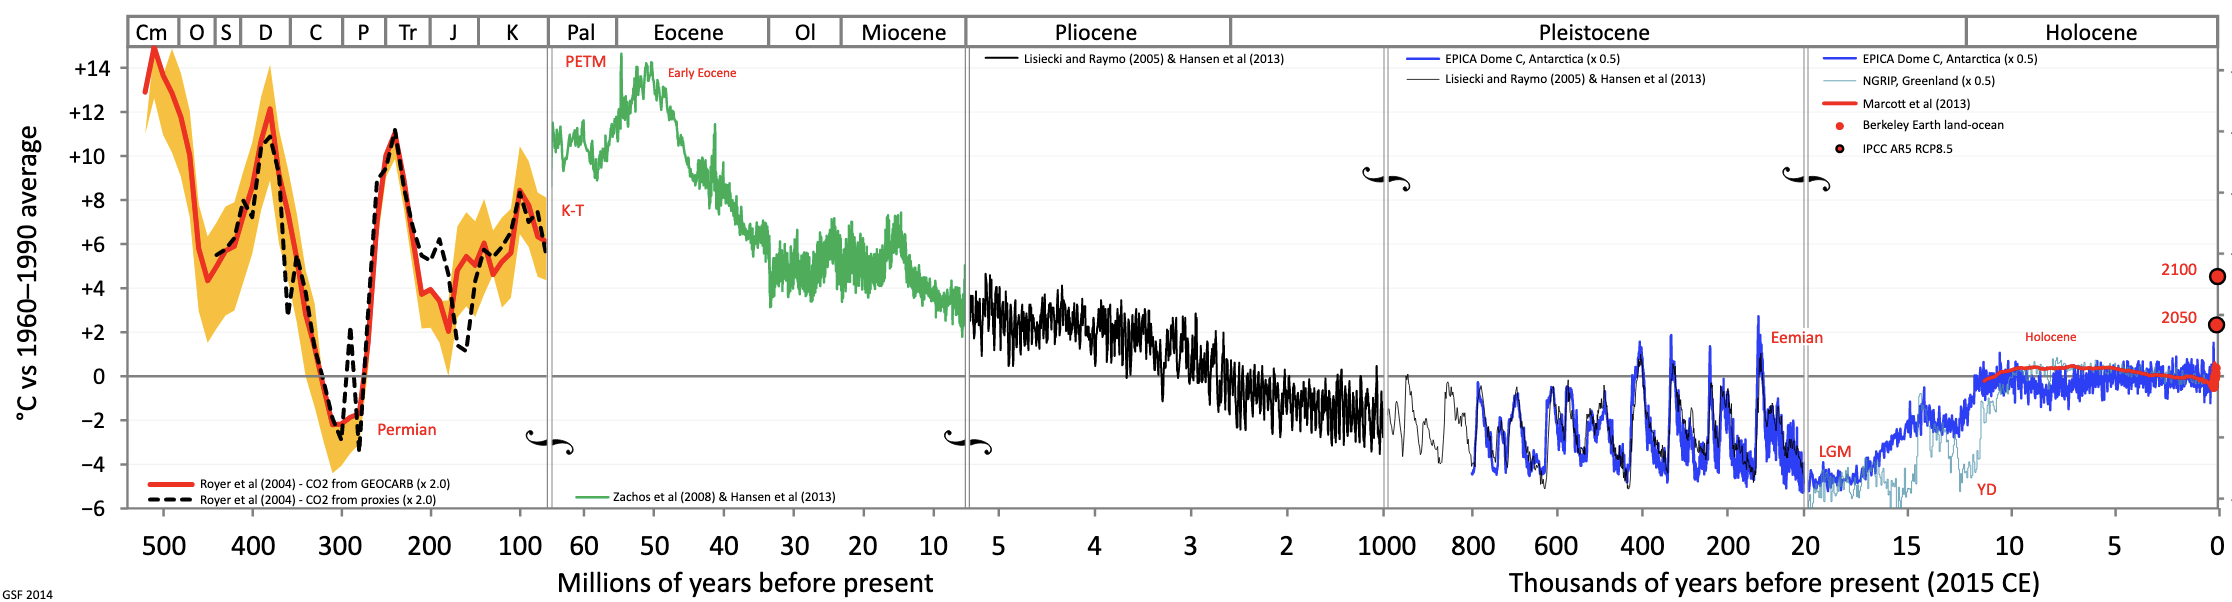
\includegraphics[width=\textwidth]{./Bilder/Paleoklima_Wiki.png}
\caption{\label{fig_PaleoTemp}%
Globale Durchschnittstemperatur auf der Erde w\"ahrend der letzten 540 Millionen Jahre.
Als Referenztemperatur dient die Durchschnittstemperatur zwischen 1960 und 1990. 
PETM: Pal\"aoz\"an/Eoz\"an-Temperaturmaximum; \glqq Permian\grqq\ bezieht sich auf
ein gro\ss es Massensterben von Pflanzen und Tieren, das vermutlich mit vulkanischen
Aktivit\"aten in Sibirien und einem vergleichsweise raschen Klimawandel einherging; \glqq Eemian\grqq\
bezieht sich auf die letzte Warmzeit (die Eem-Warmzeit) vor der letzten Kaltzeit; LGM: 
\glqq last glacial maximum\grqq\ bezeichnet das Maximum der letzten Kaltzeit; YD: \glqq
Younger Dryas\grqq, die J\"ungere Dryaszeit bezeichnet eine kurze K\"alteperiode, nachdem
die letzte Kaltzeit beendet war und ein Temperaturanstieg eingesetzt hatte; das Holoz\"an
ist die momentane Serie bzw.\ Epoche, die nach der letzten Kaltzeit einsetzte. (aus \cite{Wiki_Paleo})}
\end{figure}    

Man erkennt aber auch, dass es (z.B.\ vor rund 300 Millionen Jahren) schon mal 
K\"alteperioden\index{Eiszeit}\index{Kaltzeit}\index{Warmzeit}
gab, die mit unserer Eiszeit vergleichbar waren.\footnote{Nach der wissenschaftlichen Terminologie leben
wir heute in einer Eiszeit bzw.\ einem Eiszeitalter, wohingegen das, was wir umgangssprachlich als Eiszeit bezeichnen, 
nochmals als Kaltzeit (glacial) innerhalb einer Eiszeit gilt. Wir leben heute in einer Warmzeit (interglacial) 
innerhalb einer Eiszeit.
Die Definition von Eiszeitalter richtet sich danach, ob polare Regionen gro\ss fl\"achig vereist sind, wobei
manche Definitionen nur eine vereiste Region erfordern -- wir leben dann seit rund 34 Millionen Jahren
in einer Eiszeit -- w\"ahrend andere verlangen, dass Nord- und S\"udpol gro\ss fl\"achige 
Vereisungen zeigen -- danach leben wir seit 2,6 Millionen Jahren in einer Eiszeit.} Es gibt die Theorie
der \glqq Schneeballerde\grqq\ (snowball earth), wonach\index{Schneeballerde} 
insbesondere vor rund 600-700 Millionen Jahren die
Erde extreme K\"alteperioden durchgemacht hat, bei denen gro\ss e Teile der Erde (umstritten ist, ob
m\"oglicherweise die gesamte Erde, einschlie\ss lich vollst\"andig zugefrorener Ozeane) unter einer
Eisdecke lagen. 

\subsection{Proxies}

Proxies sind \glqq Stellvertreter\grqq. In der Pal\"aoklimatologie\index{Proxy} 
bezeichnen sie Parameter, die heute
bestimmt werden k\"onnen (z.B.\ das Verh\"altnis von ${}^{18}{\rm O}$ zu ${}^{16}{\rm O}$-Isotopen in
Gesteinsproben oder Fossilien) und von denen man gute Gr\"unde hat anzunehmen, dass sie
mit relevanten Parametern in der Vergangenheit korreliert sind (in diesem Fall z.B.\ mit der Oberfl\"achentemperatur
der Meere). 

Die Aufzeichnung bestimmter Parameter wie\index{Atmosph\"are!CO2@${\rm CO}_2$-Gehalt} 
Temperatur, ${\rm CO}_2$-Gehalt der Atmosph\"are, 
Solarkonstante etc.\ mit wissenschaftlichen Instrumenten hat erst in j\"ungerer Zeit begonnen. 
Daher erhebt sich die Frage, woher wir wissen (oder zu wissen glauben), welche Temperatur 
(${\rm CO}_2$-Gehalt, Methangehalt, Solarkonstante, etc) die Erde vor vielen Tausend bzw.\
Millionen Jahren hatte. Wenige Parameter k\"onnen wir mehr oder weniger direkt bestimmen:
Beispielsweise k\"onnen wir aus Eisbohrungen in der Antarktis in eingeschlossenen Luftblasen
direkt den ${\rm CO}_2$-Gehalt zu bestimmten vergangenen Zeiten in der Antarktis bestimmen. Auch andere
Parameter im Zusammenhang mit der chemischen Zusammensetzung der Luft lassen sich so bestimmen. 
Diese Messungen reichen maximal 800\,000 Jahre zur\"uck. Die meisten Parameter in weit
zur\"uckliegenden Zeiten werden jedoch indirekt gemessen. 

Typische Proxies sind bzw.\ finden sich in: Baumringen, Eisbohrkernen, Korallen, Ozeansedimenten, Fossilien, 
Gesteinsproben, etc.
Die folgenden Abschnitte sind nur Beispiele. Es gibt unz\"ahlige Proxies und in den meisten F\"allen
ist die Beziehung zwischen den heute gemessenen Werten und dem Parametern, auf die in fr\"uheren 
Zeiten geschlossen wird, sehr komplex. Die folgende Liste ist daher nur eine exemplarische
Auswahl. 

\subsubsection{Meeresoberfl\"achentemperatur (SST -- sea surface temperature)}

\begin{enumerate}
\item
$\delta {}^{18}{\rm O}$ ist ein Ma\ss\ f\"ur das\index{deltaO@$\delta {}^{18}{\rm O}$}\index{Meeresoberfl\"achentemperatur} 
Verh\"altnis von ${}^{18}{\rm O}$- zu\index{SST -- Sea Surface Temperature} 
${}^{16}{\rm O}$-Sauerstoffisotopen in unterschiedlichen Materialien. Definiert ist dieses 
Verh\"altnis durch
\begin{equation}
                            \delta {}^{18}{\rm O} = \frac{\Delta {\rm O}}{\Delta {\rm O}_{\rm St}} - 1 \, ,
\end{equation}
wobei $\Delta {\rm O} = \frac{{}^{18}{\rm O}}{{}^{16}{\rm O}}$ das Verh\"altnis von ${}^{18}{\rm O}$-Isotopen
zu ${}^{16}{\rm O}$-Isotopen in einer Probe ist und $\Delta {\rm O}_{\rm St}$ ein Standardwert f\"ur dieses
Verh\"altnis (definiert zu $1/498,7$, siehe \cite{Wiki_Vienna_Standard}). 

Das Isotop ${}^{18}{\rm O}$ ist schwerer als das Isotop ${}^{16}{\rm O}$. Daher verdunsten Wassermolek\"ule,
die das Isotop ${}^{18}{\rm O}$ enthalten, etwas schlechter als Wassermolek\"ule mit dem Isotop
${}^{16}{\rm O}$. F\"ur Oberfl\"achenmeerwasser in den Tropen ist das Verh\"altnis von
Wassermolek\"ulen mit ${}^{18}{\rm O}$ zu solchen mit ${}^{16}{\rm O}$ im Vergleich zu einem Standard
gr\"o\ss er. Regenwasser sowie Gebirgsb\"ache enthalten mehr ${}^{16}{\rm O}$. Diese Verh\"altnisse
h\"angen von der Temperatur ab und daher bildet $\delta {}^{18}{\rm O}$ ein Proxy f\"ur
die Oberfl\"achentemperatur von Wasser. 

Dies macht sich an manchen
Sedimenten bemerkbar. Insbesondere beobachtet man aber auch unterschiedliche Verh\"altnisse
in den karbonathaltigen Schalen bei sogenannten\index{Foraminiferen} 
Foraminiferen -- Mikroorganismen in Gew\"assersedimenten --, 
je nachdem welche Wassertemperatur 
zum jeweiligen Zeitpunkt der Schalenbildung herrschte. Das sogenannte Benthan (benthic) $\delta {}^{18}{\rm O}$ 
(Benthan, bzw.\ Englisch benthic, bezieht sich auf die obersten Schichten eines Gew\"assers) ist eines der wichtigsten
Proxies bei der Bestimmung von Temperaturen in vergangenen Zeiten.

\"Ahnliche Verh\"altnisse werden auch f\"ur\index{deltaN@$\delta {}^{15}{\rm N}$}\index{deltaC@$\delta {}^{13}{\rm C}$} 
andere Isotope definiert, beispielsweise $\delta {}^{15}{\rm N}$
(dem Isotopenverh\"altnis von ${}^{15}{\rm N}$ zu ${}^{14}{\rm N}$) und $\delta {}^{13}{\rm C}$
(dem Verh\"altnis von ${}^{13}{\rm C}$ zu ${}^{12}{\rm C}$). Diese Isotopenverh\"altnisse geben 
beispielsweise Aufschluss \"uber den Stickstoffgehalt in der Atmosph\"are oder von Wasser bzw.\
dem Methangehalt in der Atmosph\"are. 

\item
TEX${}_{86}$ steht\index{TEX${}_{86}$} 
f\"ur \glqq Tetraeder-Index von 86 Kohlenstoffatomen\grqq\  und ist eine Methode zur
Bestimmung von Meeresoberfl\"achentemperaturen in fr\"uheren Zeiten.  

Bestimmte mikroskopische Meeresorganismen (sogenannte mesophile marine Thaumarchaeota) 
besitzen eine Zellmembran, in denen sich sogenannte Glycerol-Dialkyl-Glycerol-Tetraethern-Molek\"ule 
-- GDGTs -- befinden. Diese Molek\"ule besitzen eine unterschiedliche Anzahl von Cyclopentyl-Komponenten,
das sind Ringe mit 5 C-Atomen. Die Anzahl dieser 5er-Ringe (typischer Weise zwischen 0 und 4) bzw.\ die
Mengenverh\"altnisse der GDGTs zu verschiedenen Ringzahlen h\"angen
von der Oberfl\"achentemperatur des Meeres zu dem Zeitpunkt ab, 
als sich diese Organismen gebildet haben, und dienen somit als Proxy f\"ur die Meeresoberfl\"achentemperatur. 
\end{enumerate}

\subsubsection{Sonnenaktivit\"at}

Proxies f\"ur die Sonnenaktivit\"at sind die Verh\"altnisse von ${}^{10}{\rm Be}$-Isotopen und
${}^{14}{\rm C}$-Isotopen zu ihren 
Standardisotopen.\index{Proxy!Sonnenaktivit\"at}\index{14-C@${}^{14}C}\index{10-Be@${}^{10}Be} 
Wie schon erw\"ahnt entstehen diese Isotope haupts\"achlich durch die kosmische Strahlung
in der Atmosph\"are der Erde. Der Einfluss der kosmischen Strahlung h\"angt wiederum
von der Sonnenaktivit\"at ab: Je h\"oher die Sonnenaktivit\"at, umso intensiver sind die Sonnenwinde,
die wiederum die kosmische Strahlung von der Erde teilweise ablenken. Je h\"oher die
Sonnenaktivit\"at, umso geringer ist die Intensit\"at der kosmischen Strahlung in den oberen 
Atmosph\"arenschichten und entsprechend geringer ist die Produktion von ${}^{10}{\rm Be}$-Isotopen und
${}^{14}{\rm C}$-Isotopen in diesen Schichten. Die Schwankungen in diesen Isotopen l\"asst sich
in verschiedenen Substanzen nachweisen und gibt daher einen Aufschluss \"uber die
Sonnenaktivit\"at in vergangenen Jahrtausenden bzw.\ Jahrmillionen. 

\subsubsection{Niederschlagsmengen und Sonnenscheindauer}

Die Niederschlagsmengen -- die Menge und H\"aufigkeit von Regenwasser -- hat einen Einfluss
auf die Stalagmiten in Tropfsteinh\"ohlen:\index{Niederschlagsmenge!Proxy}\index{Stalagmiten} 
Je h\"oher die Niederschlagsmenge umso mehr 
Wasser tr\"agt zur Bildung der Stalagmiten bei und umso breiter sind die B\"ander, die als
eine Form von \glqq Jahresringen\grqq\ beobachtet werden k\"onnen. 
Zumindest f\"ur die\index{Jahresringe}
letzten paar Tausend Jahre kann man so die Niederschlagsmengen eines Jahres
rekonstruieren. 

Ein anderes Proxy f\"ur die Niederschlagsmenge bzw.\ die Sonnenscheindauer in einem
Jahr sind die Jahresringe in alten B\"aumen. Auch bei manchen Schalentieren (Schnecken, Muscheln)
kann man aus den Ringstrukturen in den Schalen R\"uckschl\"usse auf das Wetter oder auch
andere Wachstumsbedingungen ziehen.
Solche Ringstrukturen findet man teilweise auch in Fossilien, sodass man Proxies aus sehr
weit zur\"uckliegenden Zeiten der Erdgeschichte hat. 

\subsubsection{Kohlendioxid-, Stickstoff- und Methangehalt in der Atmosph\"are}

F\"ur die vergangenen 800\,000 Jahre lassen sich die ${\rm CO}_2$-, ${\rm N}_2$- und
${\rm CH}_4$-Konzentrationen in der\index{Atmosph\"are!CO2@${\rm CO}_2$-Gehalt} 
Atmosph\"are mehr oder weniger direkt aus\index{CO2@${\rm CO}_2$-Gehalt!in fr\"uheren Zeiten}
Eiskernbohrungen in der Antarktis bestimmen (siehe Abb.\ \ref{fig_CO2}).

\begin{figure}[htb]
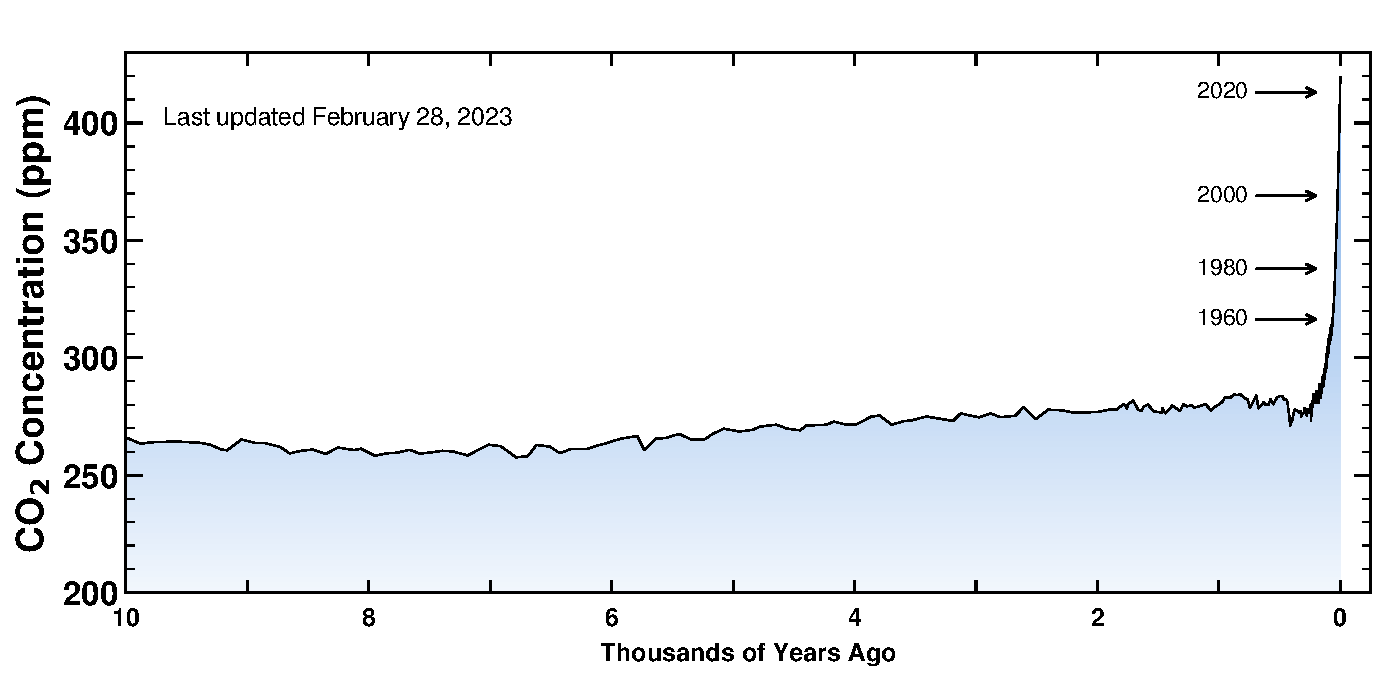
\includegraphics[width=0.49\textwidth]{./Bilder/co2_10k.pdf}
\hfill
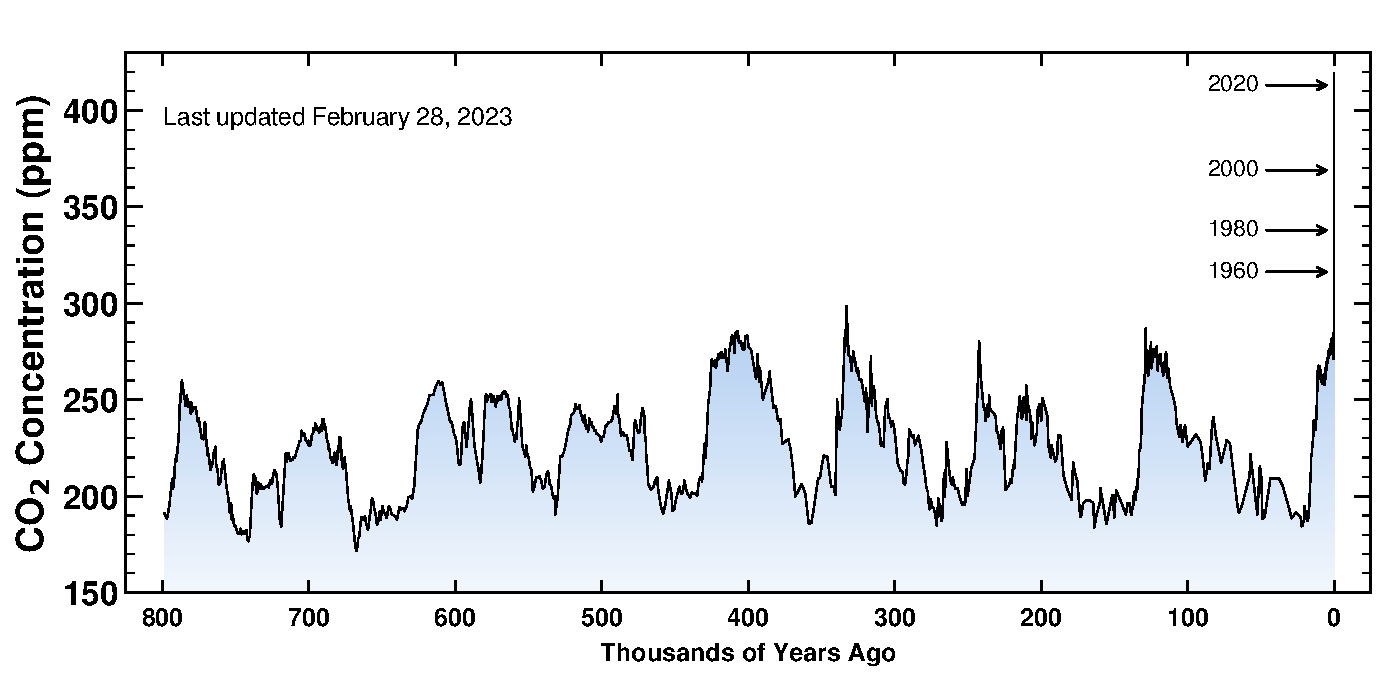
\includegraphics[width=0.49\textwidth]{./Bilder/co2_800k.pdf}
\caption{\label{fig_CO2}%
Der ${\rm CO}_2$-Gehalt in der Atmosph\"are, bestimmt aus Eiskernbohrungen in der
Antarktis. (links) f\"ur die vergangenen 10\,000 Jahre, (rechts) f\"ur die vergangenen
800\,000 Jahre.}
\end{figure} 

Man erkennt auf diesen Bildern sehr gut die sogenannte Hockeyschl\"agerkurve der
${\rm CO}_2$-Konzentration in den letzten 10\,000 Jahren nach der letzten Kaltzeit sowie
die Schwankungen zwischen Kaltzeiten und Warmzeiten innerhalb der letzten
800\,000 Jahre. Mit etwas Phantasie
erkennt man auch einen leichten Anstieg der ${\rm CO}_2$-Konzentrationen vor rund
6--8 Tausend Jahren, der mit dem Beginn von Viehzucht, Ackerbau und generell der
Sesshaftigkeit des Menschen einhergeht: Es wurden Weide- und Ackerbaufl\"achen 
abgebrannt und somit erste fossile Brennstoffe freigesetzt. Au\ss erdem haben beispielsweise
der Anbau von Reis auf gro\ss fl\"achigen Reisterrassen sowie die Viehzucht
die Freisetzung von Methan, einem weiteren Treibhausgas, gef\"ordert. Dieser Trend hat jedoch
lediglich dazu gef\"uhrt, dass eine einsetzende neue Kaltzeit etwas verz\"ogert wurde. 
Erst der Beginn der industriellen Revolution und der damit verbundene intensive Verbrauch
fossiler Brennstoffe vor rund 200 Jahren hat den ${\rm CO}_2$-Gehalt der Luft deutlich
ansteigen lassen. 

\section{Der Meeresspiegel} 

Eine\index{Meerespiegel!Proxy}\index{Meeresspiegel!in fr\"uheren Zeiten} 
der drastischsten Folgen eines Klimawandels ist der Anstieg des Meeresspiegels. 
Auch hier gibt es nat\"urlich viele Untersuchungen \"uber den Meeresspiegel in der
Vergangenheit. Beispielsweise war der Meerespiegel w\"ahrend der letzten Kaltzeiten
um rund 120 Meter niedriger als heute (siehe Abb.\ \ref{fig_PaleoSea}).

\begin{SCfigure}[30][htb]
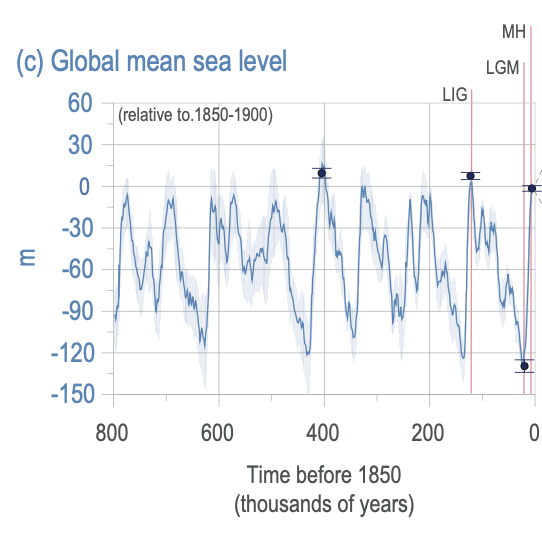
\includegraphics[width=0.4\textwidth]{./Bilder/Paleo_Sea_Level.png}
\caption{\label{fig_PaleoSea}%
Der mittlere Meerespiegel in den letzten 800\,000 Jahren relativ zu der
Zeitperiode 1850--1900. Deutlich erkennbar ist, dass der Meeresspiegel 
w\"ahrend der Kaltzeiten um \"uber 100 Meter niedriger war als heute. Allerdings war
der Meeresspiegel w\"ahrend der letzten Warmzeiten auch teilweise einige
Meter h\"oher. LIG last interglacial, LGM last glacial maximum, MH mid-Holocene.
(aus \cite{IPCC_WG1_AR6})}
\end{SCfigure}

Allerdings war er w\"ahrend der letzten Warmzeiten auch einige Meter
h\"oher als heute. Im Wesentlichen sind zwei Faktoren f\"ur die H\"ohe des 
Meeresspiegels verantwortlich: (1) die Temperatur des Wassers und (2) die
Menge an landgebundenem Eis. Die Temperatur des Wassers hat einen
Einfluss auf die Ausdehnung. Der Volumenausdehnungskoeffizient von Wasser
bei $20^\circ$C betr\"agt ungef\"ahr $\gamma = 0,2 \cdot 10^{-3} {\rm K}^{-1}$. Eine 
Wassers\"aule von 4\,000\,m (durchschnittliche Tiefe des Ozeans) w\"urde sich
bei einer Erw\"armung um 1 Grad Celsius somit um rund 80\,cm ausdehnen. 
Das gibt eine Vorstellung von der Gr\"o\ss enordnung. Nat\"urlich erw\"armt sich
das Wasser nicht gleich bis in eine Tiefe von 4\,km, andererseits betr\"agt die
langfristige Erw\"armung an der Oberfl\"ache vermutlich mehr als ein Grad. 

Der zweite
Faktor ist entscheidender: Da die Gesamtwassermenge an der Erdoberfl\"ache (Ozeane,
Land und Atmosph\"are) ungef\"ahr konstant ist, sinkt der Meeresspiegel,
wenn gro\ss e Landstriche (Antarktis, Gr\"onland, Alaska und Kanada, Nordeuropa,
etc.) mit Eis bedeckt sind. Bei der letzten Kaltzeit war Europa bis zu den Alpen mit
einer dicken Eisschicht bedeckt. Dies macht den gr\"o\ss ten Anteil der Schwankungen
in der Meeresh\"ohe aus. Schwimmendes Eis, wie es teilweise in der Arktis vorliegt, hat
aufgrund des archimedischen Prinzips
nat\"urlich keinen Einfluss auf die Wasserh\"ohe, 

Als Proxy f\"ur die Meereh\"ohe dienen oftmals bestimmte Fossilien im Sediment bzw.\
in Gesteinsproblem, von denen bekannt ist, dass sie nur in seichtem Meerwasser
leben. 

Die Pal\"aoklimatologie zeigt somit, dass wir in der Vergangenheit
sehr unterschiedliche klimatische Verh\"altnisse auf der Erde hatten. Man kann kaum
irgendein Klima als \glqq f\"ur die Erde normal\grqq\ bezeichnen. Einen wesentlichen Einfluss
hatten dabei die Kontinentalverschiebungen: Diese f\"uhrten zu ver\"anderten Str\"omungsverh\"altnissen
der Ozeane, zu teilweise erh\"ohten vulkanischen Aktivit\"aten mit massivem ${\rm CO}_2$ Aussto\ss, zum
Aufbau von Gebirgen wie dem Himalaya (bei diesen Prozessen werden gro\ss e Mengen
an ${\rm CO}_2$ durch Verwitterungsprozesse gebunden), etc. Ein weiterer Faktor waren
gro\ss e Meteoriteneinschl\"age, die in der fernen Vergangenheit h\"aufiger stattfanden als heute. 

Der Einfluss des Menschen\index{Klimawandel!anthropogener}
in j\"ungerer Zeit ist mittlerweile unbestritten. Letztendlich wird der anthropogene Klimawandel
den Planten Erde nicht zerst\"oren -- die Evolution wird neue, dem Klima angepasste Lebensformen
hervorbringen -- aber wir zerst\"oren den Lebensraum, in dem wir Menschen entstanden sind
und gleichzeitig werden viele vertraute Lebensformen aussterben, die im Zuge der k\"uhleren
letzten 20--30 Millionen Jahre entstanden sind. Viele derzeit bewohnte Gebiete werden im
Meer versinken und die H\"aufigkeit von Trockenzeiten und anderen extremen Wetterverh\"altnissen
werden zunehmen. Die Folgen des gr\"o\ss ten Problems -- die mit dem Klimawandel verbundene
Migration von Milliarden von Menschen -- sind dabei derzeit kaum absehbar. 
 

\section{Anmerkungen}

\begin{anmerkungen}
\item
\label{Anm-1}%
Der Grund f\"ur den Faktor 2 zwischen der Schwankung im Abstand und
der Schwankung in der Intensit\"at der Sonneneinstrahlung liegt in dem $1/r^2$-Gesetz
der Intensit\"at als Funktion des Abstands:
\begin{equation}
        \frac{1}{(r\pm \Delta r)^2} \approx \frac{1}{r^2} \mp 2 \frac{\Delta r}{r} \, .
\end{equation}

\end{anmerkungen}



\begin{thebibliography}{99}
\bibitem{ICS} International Commission on Stratigraphy (ICS) \url{https://stratigraphy.org/chart}. 
\bibitem{IPCC_WG1_AR6} IPCC -- Climate Change 2021; The Physical Science Basis, 
            Full Report, Working Group I Contribution to the Sixth Assessment Report (S.\,159). 
\bibitem{NASA_World} NASA Image and Video Library, 
       \url{https://images.nasa.gov/details/as17-148-22727}
\bibitem{NASA_facts} NASA Earth Fact Sheet; 
      \url{https://nssdc.gsfc.nasa.gov/planetary/factsheet/earthfact.html}   
\bibitem{Solar} Solarkonstante; Uni Kassel,\\
       \url{https://www.greenrhinoenergy.com/solar/radiation/images/solar-constant.jpg}         
\bibitem{Wikipedia_Faint} Wikipedia \glqq Faint young Sun paradox\grqq\ 
        \url{https://en.wikipedia.org/wiki/Faint_young_Sun_paradox}.                 
\bibitem{Wikipedia_Milankovic} Wikipedia \glqq Milankovitch cycles\grqq.   
       \url{https://en.wikipedia.org/wiki/Milankovitch_cycles}.      
\bibitem{Wiki_Paleo} Wikipedia \glqq Paleoclimatology\grqq\ \url{https://en.wikipedia.org/wiki/Paleoclimatology}.         
\bibitem{Wikipedia_Solarkonstante} Wikipedia \glqq Solarkonstante\grqq.   
       \url{https://de.wikipedia.org/wiki/Solarkonstante}.    
\bibitem{Wiki_Vienna_Standard} Wikipedia \glqq Vienna Standard Mean Ocean
         Water\grqq\ \url{https://de.wikipedia.org/wiki/Vienna_Standard_Mean_Ocean_Water}.                  
\end{thebibliography}

\end{document}

